\chapter{Результаты исследования}

Были рассмотрены три меры схожести пользователей --- косинусное сходство, коэффициент Жаккара и коэффициент корреляции Пирсона. Для оценки влияния каждой меры схожести пользователей на качество рекомендаций рассчитывался показатель ROC-AUC. Для этого задача сводилась к бинарной классификации при сравнении предсказанных рекомендаций на основании обучающей выборки (случайного подмножества игр, в которые играл пользователь и на основании которых можно подобрать похожих пользователей) и истинных предпочтений игрока (всего множества игр, в которые играл пользователь): 1, если пользователь поиграл в рекомендованную игру, 0 иначе.

Исследование проводилось на пользователях, которые играли более чем в 5 игр. На рисунке \ref{img:1} представлена зависимость качества рекомендаций от меры схожести пользователей и числа ближайших соседей K, по которым подбирались рекомендации.

\begin{figure}
	\begin{center}
		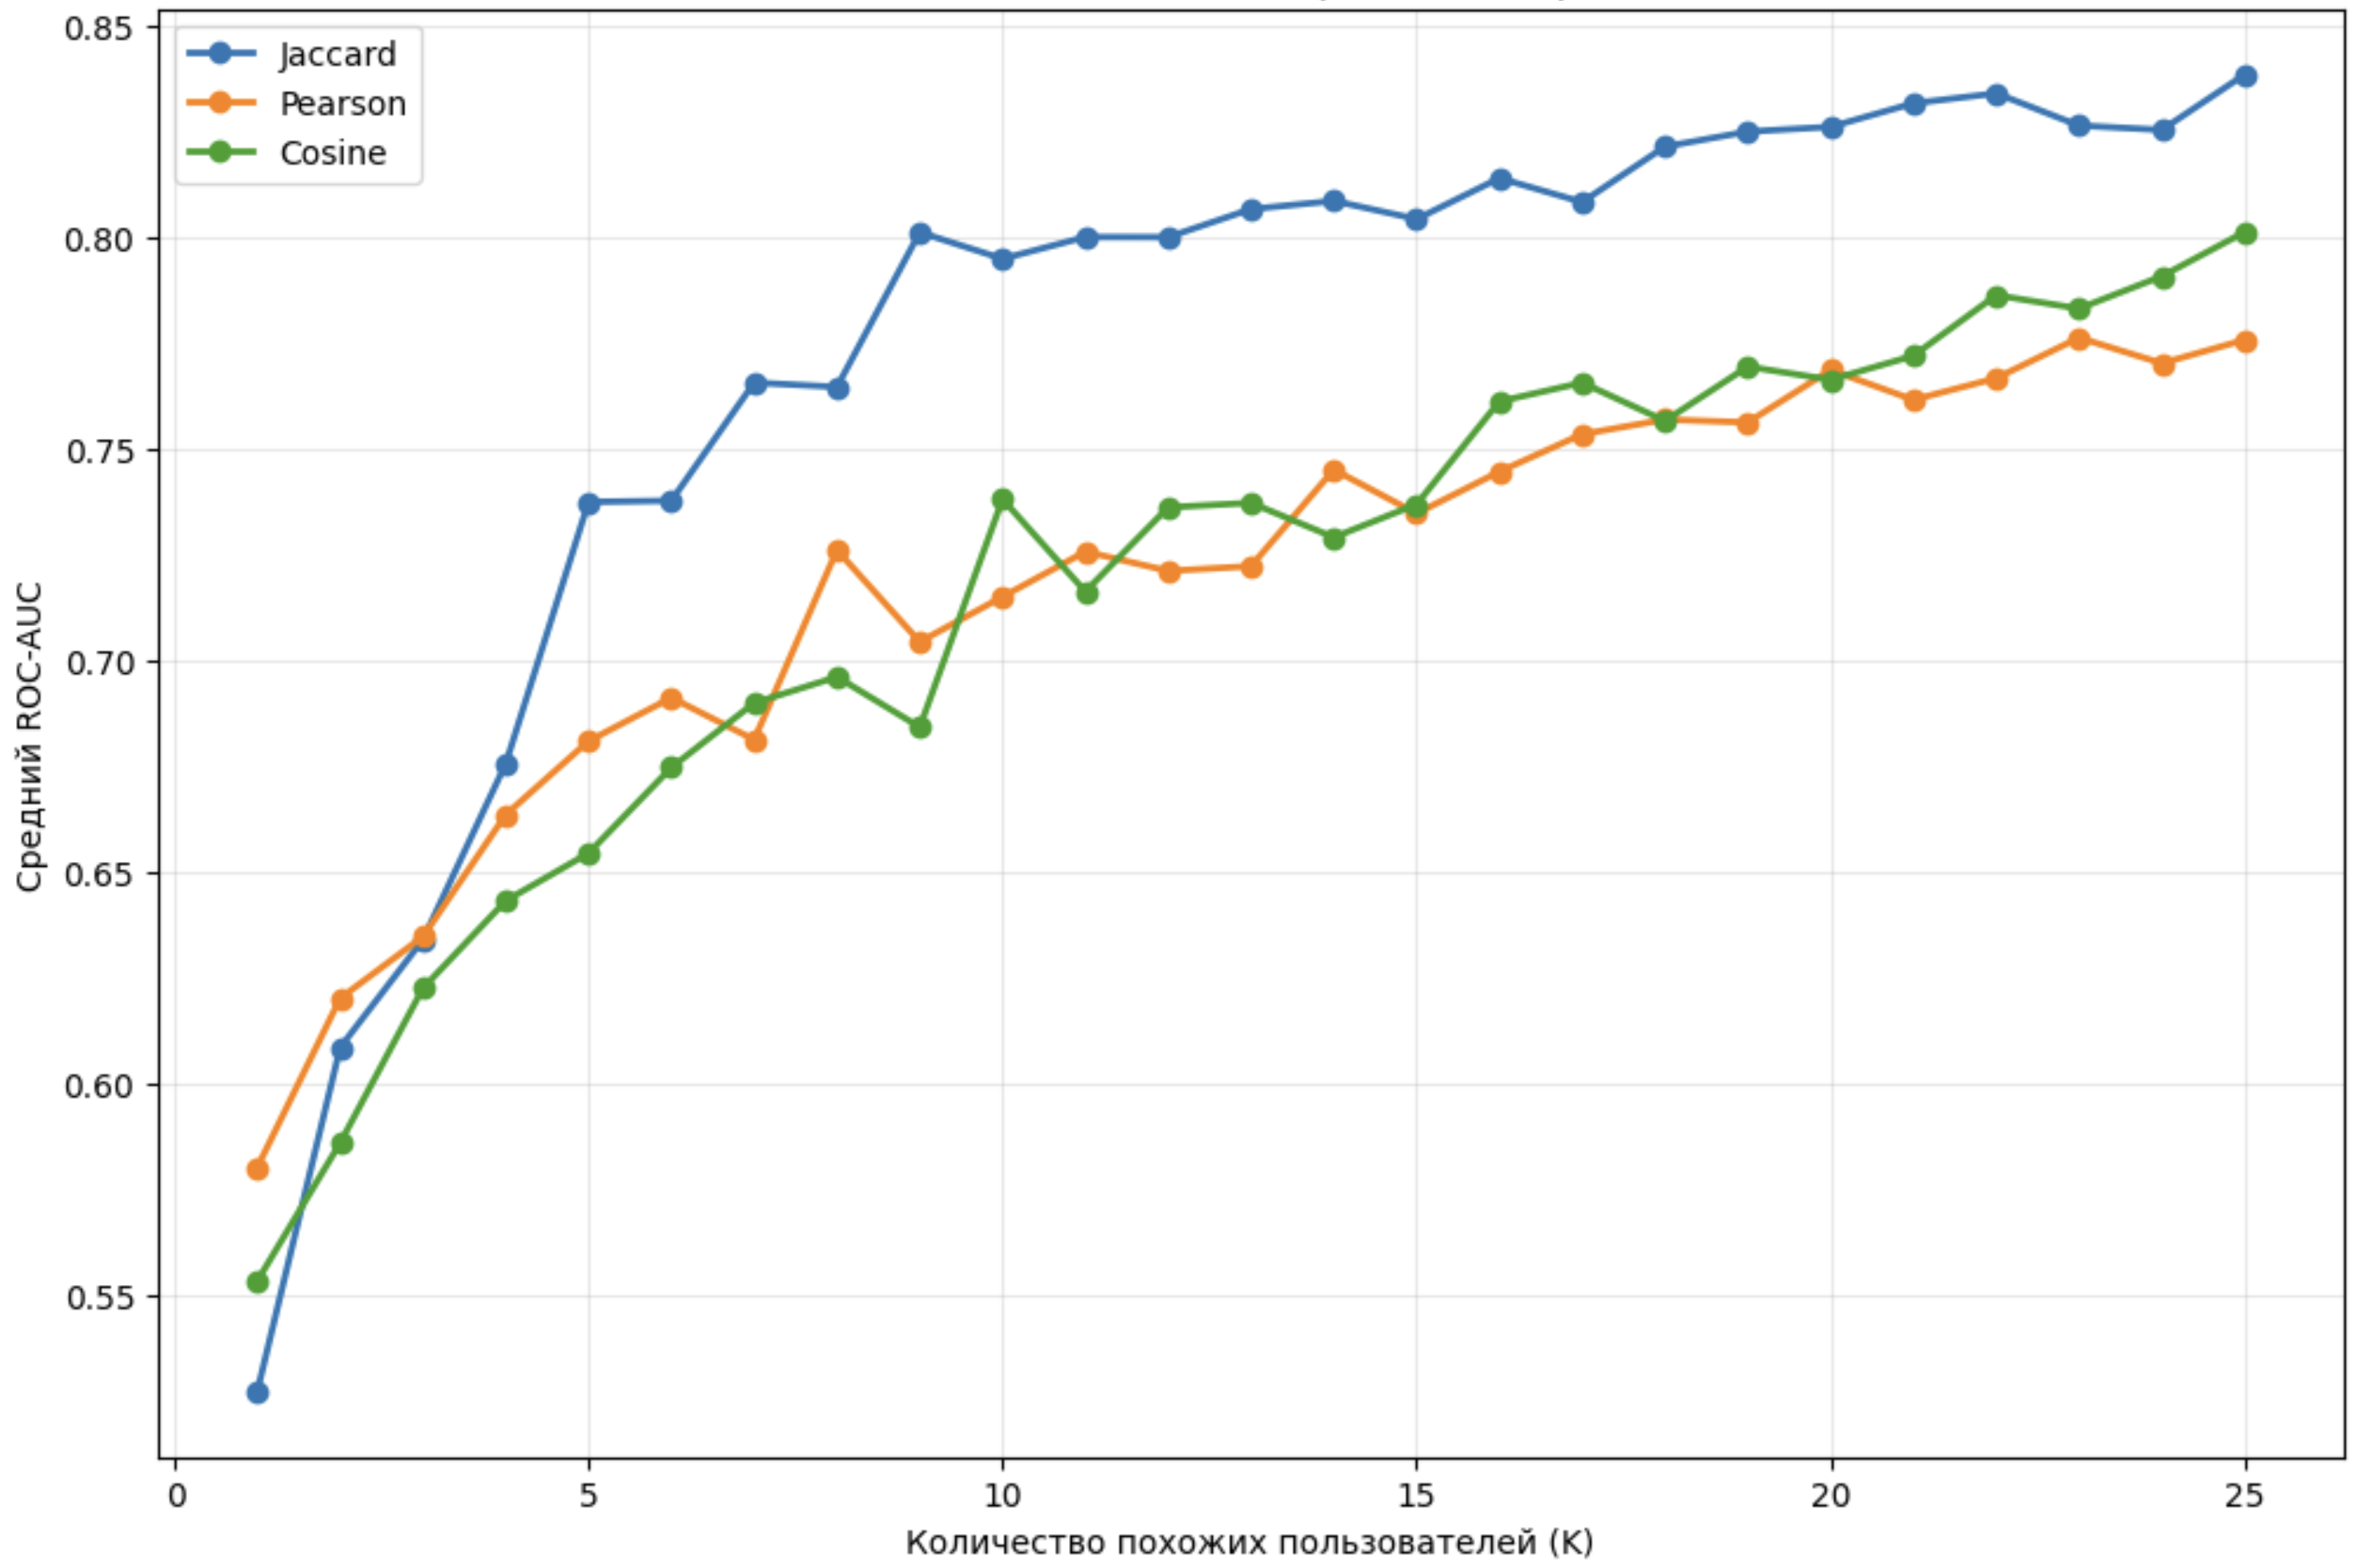
\includegraphics[width=\textwidth]{images/1.png}
	\end{center}
	\caption{Зависимость метрики ROC-AUC от количества похожих пользователей для разных мер схожести}
	\label{img:1}
\end{figure}

\clearpage
